\chapter{Introduction to Deep Learning}

Deep Learning is a subset of Machine Learning involving algorithms that closely model the human brain and through multi-layer neural networks. Such layers can perform of feature extraction and transformation, learning complex patterns in large amounts of data, automating the manual pre-processing done in typical Machine Learning.
\begin{figure}[H]
    \centering
    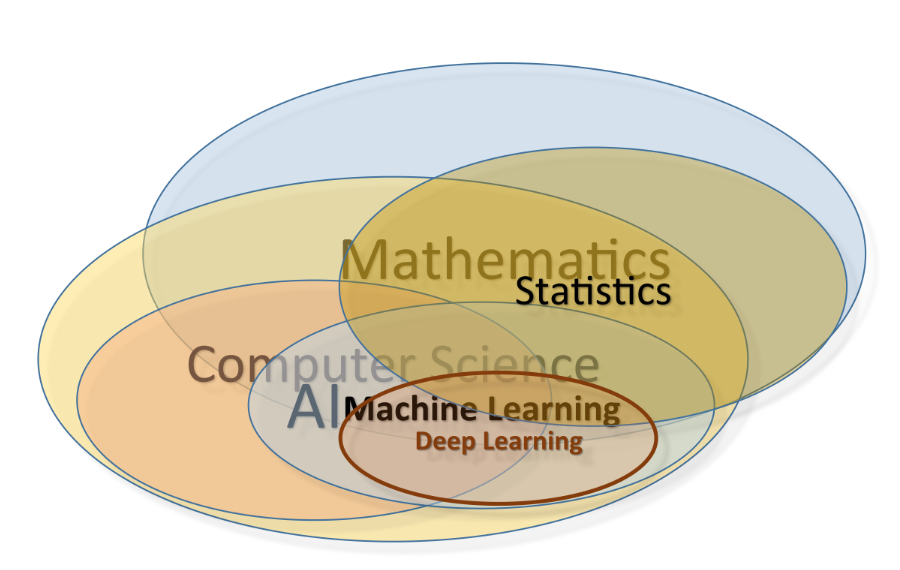
\includegraphics[width=0.3\linewidth]{img/overlap.png}
\end{figure}

\begin{figure}[H]
    \centering
    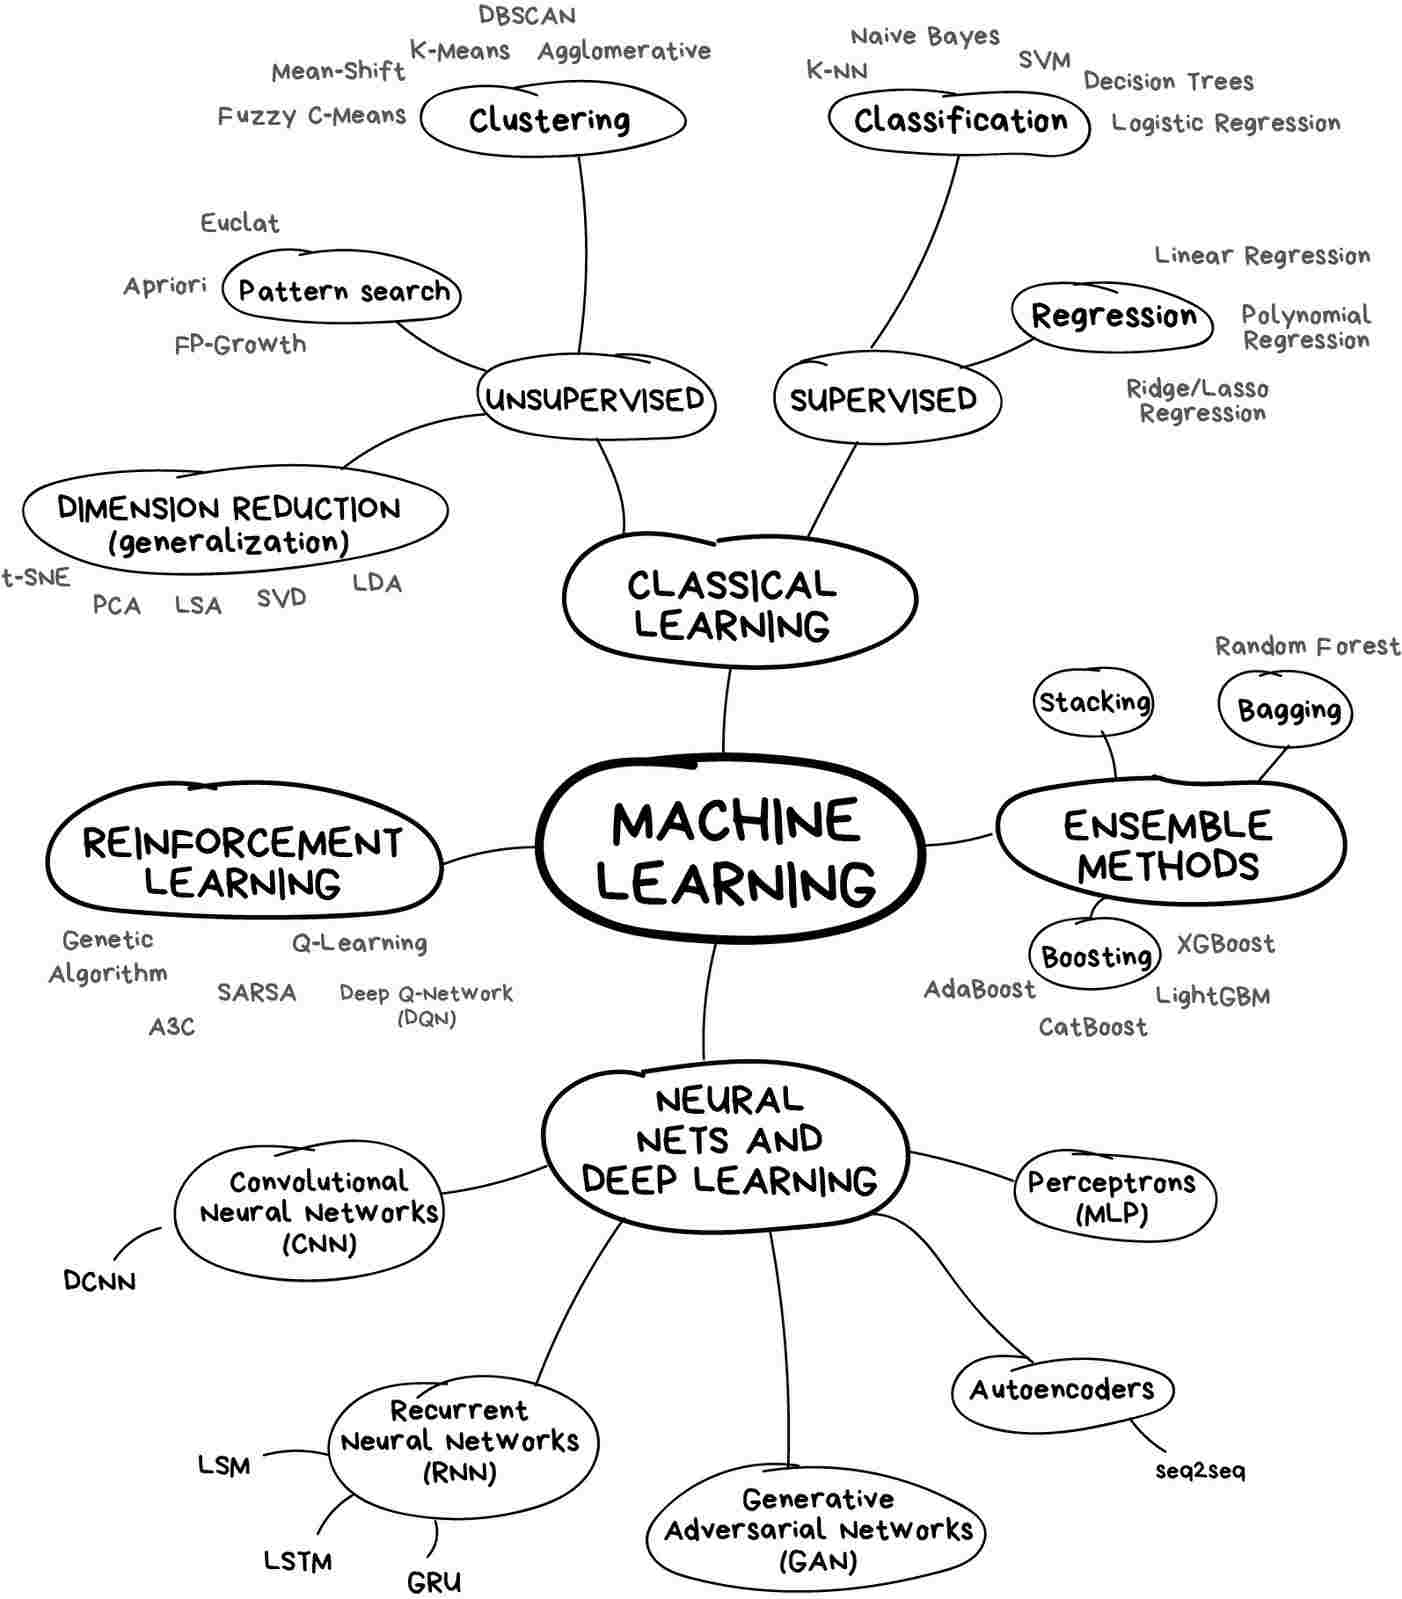
\includegraphics[width=0.55\linewidth]{img/ml_flowchart.png}
    \caption{Image Credit: Data Revenue}
    
\end{figure}

\section{Machine Learning Recap}
\subsection{Problem Formulation}
\textbf{Input}: \\
Let $x$ be the input, where $x\in\mathcal{X}\subset\mathcal{D}$. In practical applications, this input could be in various forms such as a piece of text, an image, an audio clip, or data from a sensor output.\\

\textbf{Output}: \\
The output is denoted as $\mathbf{y}$, where $\mathbf{y}\in\mathcal{Y}$. $\mathcal{Y}$ is the set of all possible outputs This is typically a label or a predicted outcome based on the given input.\\

\textbf{Experience \(\mathcal{X}\)}: \\
This refers to the observations or the training data set that falls within domain \(D\). The data points are denoted as \(x \in \mathcal{X} \subseteq D\). The pairs \((x_1, y_1), (x_n, y_n)\) denote the individual data and target output points.\\


\textbf{Target Function $f:\mathcal{X}\to\mathcal{Y}$}: \\
The target function is denoted as $f$ which maps from $\mathcal{X}$ to $\mathcal{Y}$, represented as $f:\mathcal{X}\to\mathcal{Y}$. In real-world scenarios, this true underlying function is never known in practice.\\

\textbf{Domain of Data $\mathcal{D}$}: \\
The set of all possible data points for testing or out-of-sample validation. It is represented as \(D\). Data is the fundamental component used to train models in machine learning. It is often represented as a set of input-output pairs: $(\mathbf{x}_1,y_1),(\mathbf{x}_n,y_n),\ldots,(\mathbf{x}_n,y_n)$. \\

\textbf{Error Function $\widehat{R}_n$}: \\
The error function quantifies the deviation of the predicted output from the actual output. It's represented as:
\[
\widehat{R}_n=\frac1n\sum_n\widehat{l}(g(w,x),y)
\]\\

\subsection{Error Measures and Loss Functions}
\begin{itemize}
    \item Defined by the user for the ML task
    \item Depends on the type of prediction (binary classification, regression, etc)
\end{itemize}

The training error measures the discrepancy on the dataset used to find \( h \), while the test error gives an expectation of the error on new, unseen data:

\begin{itemize}
    \item \textbf{Squared Error}: \( \ell(y, \widehat{y}) = (y - \widehat{y})^2 \)
    \item \textbf{Binary Error}: \( \ell(y, \widehat{y}) = \mathbb{I}(y \neq \widehat{y}) \)
    \item \textbf{Cross-Entropy Error:} \(\widehat R_n(\mathbf{w})=\frac1n\sum_{i=1}^n\log\left(1+e^{-y_i\mathbf{w}^\top\mathbf{x}_i}\right)\);
\end{itemize}


\begin{align*}
    \text{Training Error:} \quad & R_{\text{in}}(h) = \frac{1}{n} \sum_{i=1}^{n} \ell(h(x_i), y_i) \\
    \text{Test Error:} \quad & R(h) = \mathbb{E}[\ell(h(x), y)]
\end{align*}

$\ell$ is the error function that depends on the type of machine learning methods used.

\begin{definitionbox}{Learning Setup Overview}
    

\begin{itemize}
    \item \textbf{Input and Output:} The learning algorithm receives an input \( x \in \mathcal{X} \) and predicts an output \( y \in \mathcal{Y} \). The true relationship between inputs and outputs is governed by the unknown probability distribution \( P(y|\mathbf{x}) \), which the learning algorithm tries to approximate.
    $$ \{(x_1, y_1), (x_2, y_2), \ldots, (x_n, y_n)\}  \sim P$$
    
    \item \textbf{Data:} We collect a dataset \( \{(x_1, y_1), (x_2, y_2), \ldots, (x_n, y_n)\} \) which is assumed to be sampled from the joint distribution \( P(x, y) \). This dataset serves as the empirical basis for learning the input-output mapping.
    
    \item \textbf{Hypothesis Class:} The hypothesis class \( \mathcal{H} \) is the set of all functions \( h: \mathcal{X} \rightarrow \mathcal{Y} \) that the learning algorithm considers. The choice of \( \mathcal{H} \) can significantly impact the algorithm's ability to generalise from the training data to unseen data.
    $$
    \mathcal{H} \subset \{h(\mathbf{w}):\mathcal{X} \rightarrow \mathcal{Y}, w \in \mathbb{R}\}
    $$
    
    \item \textbf{Loss Function:} The loss function \( \ell: \mathcal{Y} \times \mathcal{Y} \rightarrow \mathbb{R} \) quantifies how far off a prediction is from the actual value. It provides a criterion for evaluating the quality of a hypothesis.
    
    \item \textbf{Learning Objective:} The goal of learning is to find a hypothesis \( \mathbf{w}^* \in \mathbb{R}^{||\mathbf{w}||} \) that best approximates the true distribution \( P(y|\mathbf{x}) \). Formally, we seek a hypothesis that minimises the expected loss over the data distribution: 
    \[\mathbf{w}^*=\operatorname*{argmin}_{\mathbf{w}}\left\{R(\mathbf{w})=\mathbb{E}\left[\ell(h(\mathbf{w}\mathbf{x}),\mathbf{y})\right]\right\}\]

\end{itemize}

\end{definitionbox}

\subsection{Neural Network Perceptron and Activation Functions}
\subsection{Gradient Descent}
The parameter update rule in gradient descent is given by:
\[ \mathbf{w}_{t+1} = \mathbf{w}_t + \eta\mathbf{v}, \]
where \( \mathbf{v} \) is the direction vector of the steepest descent, and \( \eta \) represents the learning rate.

\begin{sidenotebox}{More information on gradient descent}
If $\mathbf{v}=-\frac{\nabla\hat{R}_{n}(\mathbf{w}_{t})}{\|\nabla\hat{R}_{n}(\mathbf{w}_{t})\|}$, direction is defined by:
\begin{align*}\Delta\hat{R}_{n}&=\hat{R}_{n}(\mathbf{w}_{t+1})-\hat{R}_{n}(\mathbf{w}_{t})\\
&=\hat{R}_{n}(\mathbf{w}_{t}+\eta\mathbf{v})-\hat{R}_{n}(\mathbf{w}_{t})\\
&=\eta\nabla\hat{R}_{n}(\mathbf{w}_{t})^{\top}\mathbf{v}+O(\eta^{2})\geqslant-\eta\|\nabla\hat{R}_{n}(\mathbf{w}_{t})\|+O(\eta^{2})\end{align*}

The direction of the parameter update in gradient descent is key to effectively minimising the risk function \( \hat{R}_n \). The change in \( \hat{R}_n \) after an update is defined as:

\[ \Delta \hat{R}_n = \hat{R}_n(\mathbf{w}_{t+1}) - \hat{R}_n(\mathbf{w}_t) \]

Given the update rule \( \mathbf{w}_{t+1} = \mathbf{w}_t + \eta\mathbf{v} \), where \( \mathbf{v} \) is a unit vector and \( \eta \) is the learning rate, we can approximate the change in \( \hat{R}_n \) using a Taylor expansion:

\[ \hat{R}_n(\mathbf{w}_{t+1}) \approx \hat{R}_n(\mathbf{w}_t) + \eta \nabla \hat{R}_n(\mathbf{w}_t)^\top \mathbf{v} + O(\eta^2) \]

The optimal direction \( \mathbf{v} \) for the steepest descent is in the direction of the negative gradient, normalised:

\[ \mathbf{v} = -\frac{\nabla \hat{R}_n(\mathbf{w}_t)}{\| \nabla \hat{R}_n(\mathbf{w}_t) \|} \]

Incorporating this into the update rule, we achieve the gradient descent step:

\[ \mathbf{w}_{t+1} = \mathbf{w}_t - \eta \frac{\nabla \hat{R}_n(\mathbf{w}_t)}{\| \nabla \hat{R}_n(\mathbf{w}_t) \|} \]

This step ensures that the parameters are updated in the direction that most rapidly decreases the risk function \( \hat{R}_n \), taking into account the magnitude of the learning rate \( \eta \).
\end{sidenotebox}

\begin{definitionbox}{Backpropagation Training }
\begin{enumerate}
    \item Initialize all network weights \( w_{ij}^{(l)} \) randomly to break symmetry.
    \item For each iteration \( t = 1, 2, \ldots \) until convergence:
    \begin{enumerate}
        \item Select a data point \( (x_k, y_k) \) randomly or sequentially.
        \item \textbf{Forward Pass}:
        \begin{itemize}
            \item Compute the activation \( x_j^{(l)} \) of each layer \( l \) starting from the input layer and progressing through to the output layer.
        \end{itemize}
        \item \textbf{Backward Pass}:
        \begin{itemize}
            \item Compute the gradient of the loss function with respect to the activations \( \delta_j^{(l)} \), starting from the output layer and propagating back to the input layer.
        \end{itemize}
        \item \textbf{Update Weights}:
        \begin{itemize}
            \item Adjust the weights \( w_{ij}^{(l)} \) in the direction that most reduces the loss, typically using a learning rate \( \eta \) and the gradient \( \delta_j^{(l)} \).
            \item The update can be done using a single data point (Stochastic Gradient Descent), a minibatch of data points, or the entire dataset (batch gradient descent).
        \end{itemize}
    \end{enumerate}
    \item After sufficient iterations or upon convergence, return the final weights \( w_{ij}^{(l)} \).
\end{enumerate}
    
\end{definitionbox}

\subsection{Learning from Noisy Data}
\begin{figure}[H]
    \centering
    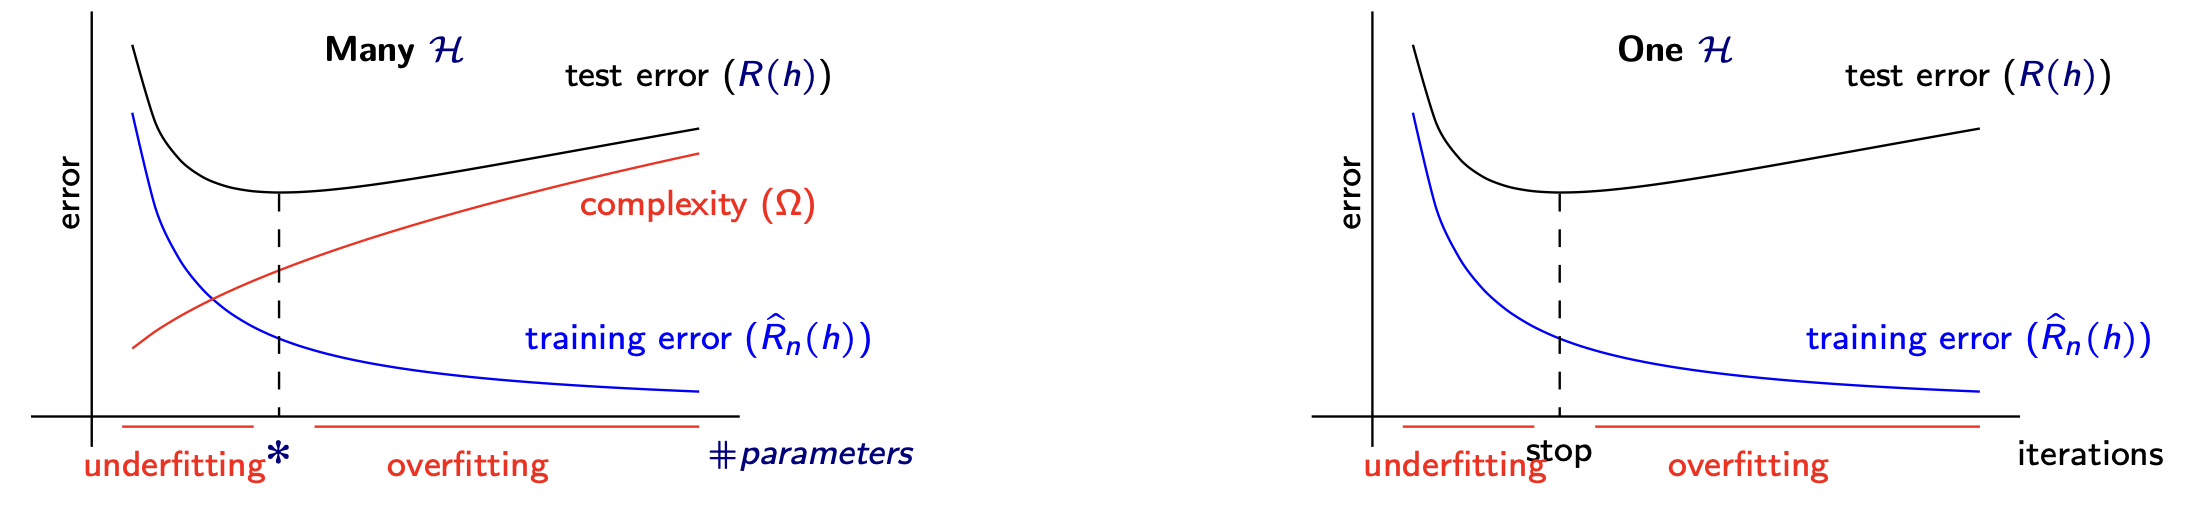
\includegraphics[width=0.5\linewidth]{img/learning_curve.png}
    \caption{Enter Caption}
    
\end{figure}

Stochastic noise comes from random errors when measuring data. Deterministic noise stems from our chosen hypothesis from training, that fails to predict certain values of the target hypothesis.\\

Overfitting occurs when the model fits to noise instead of the underlying target function, also known as the distribution. This occurs when \(\widehat{R}_n(h)\) decreases and \(R(h)\) increases, and we diverge from the target function.

Both deterministic and stochastic noise lead to overfitting – we can reduce this by increasing the number of data points.

\subsection{Regularisation}

Regularisation is used to combat overfitting, by adding a penalty term to the error.

\subsubsection*{Regularised Loss (Augmented Error)}

The regularised loss function \(\mathcal{L}_n(h)\) can be expressed as the sum of the empirical risk \(\hat{R}(h)\) and a regularisation term \(\Omega(h)\) scaled by a parameter \(\lambda\), which acts as an overfit penalty:

\[
\mathcal{L}_n(h) = \hat{R}(h) + \lambda \underbrace{\Omega(h)}_{\text{overfit penalty}}
\]

The regularisation term \(\Omega(h)\) is applied to the model parameters to enforce simplicity and robustness. Different norms can be used for \(\Omega(h)\), each with its own implications:

\begin{itemize}
    \item \(\|\mathbf{w}\|_2^2\): L2 regularisation, also known as Ridge regression, penalises the sum of the squares of the model weights.
    \item \(\|\mathbf{w}\|_1\): L1 regularisation, also known as Lasso, penalises the sum of the absolute values of the model weights, leading to sparsity.
    \item \(\|\mathbf{w}\|_1 + \|\mathbf{w}\|_2^2\): Elastic net regularisation combines L1 and L2 regularisation.
    \item \(\mathbf{w}^\top \Gamma ^\top \Gamma \mathbf{w}\): Tikhonov regularisation, a generalised form of L2 regularisation where \(\Gamma\) is a positive semi-definite matrix. \(\Gamma\) can incorporate information about the relationships between different features or can be used to impose specific structures on the solution.
\end{itemize}

\textbf{Occam's Razor:}

\begin{definitionbox}{Occam's Razor}
Occam's Razor is a philosophical principle that suggests that simpler models are usually better. They also have good generalisation capabilities, having smoother and simpler functions, because noise within the data is typically not smooth.

\end{definitionbox}

\begin{definitionbox}{Regularised Loss Minimisation (RLM)}
\subsubsection*{Hypothesis Class}

The hypothesis class \( \mathcal{H} \) is defined as a set of functions \( h \) parameterised by weight vector \( \mathbf{w} \) and regularisation parameter \( \lambda \), where \( \lambda \) controls the trade-off between fitting the error term and enforcing simplicity of the model.

\[
\mathcal{H} = \{ h_i = h(\mathbf{w}; \lambda_i) | i \in \mathbb{N} \}
\]

Here, \( \lambda_i \) takes on values from a predetermined set, such as \( \{0.0001, 0.001, \ldots\} \), allowing for the exploration of different levels of model complexity.

\subsubsection*{Augmented Error}

The augmented error \( \mathcal{L}_k(\mathbf{w}, \lambda) \) combines the empirical risk \( \hat{R}_k(\mathbf{w}) \) with a regularisation term \( \lambda\Omega(\mathbf{w}) \):

\[
\mathcal{L}_{\bar{k}}(\mathbf{w}, \lambda) = \hat{R}_{\bar{k}}(\mathbf{w}) + \lambda\Omega(\mathbf{w})\quad  \text{where }\Omega(\mathbf{w})\in\{\|\mathbf{w}\|_2^2,\|\mathbf{w}\|_1,\|\mathbf{w}\|_2^2+\|\mathbf{w}\|_1,\ldots\}
\]

where \( \hat{R}_{\bar{k}}(\mathbf{w}) \) is the average loss over the dataset and \( \Omega(\mathbf{w}) \) is a function imposing a penalty for complexity. 


\subsubsection*{RLM Solution:}

The RLM solution involves
\begin{enumerate}
    \item Training a model on dataset \( D_{\bar{k}} \) for all \( i \), using the regularised loss \( \mathcal{L}_{\bar{k}}(\mathbf{w}, \lambda_i) \), to obtain different hypotheses for different values of \( \lambda_i \):
    \[
    g(\mathbf{w}_{\lambda_i}) = \underset{\mathbf{w}}{\mathrm{argmin}}\ \mathcal{L}_{\bar{k}}(\mathbf{w}, \lambda_i)
    \]
    
    \item Selecting the best hypothesis from among these by evaluating their performance on a validation set \( D_k \), usually by measuring the empirical risk \( \hat{R}_k(g(\mathbf{w}_{\lambda_i})) \) and choosing the one with the lowest loss:
    \[
    g(\mathbf{w}_{\lambda_*}) = \underset{\lambda_i}{\mathrm{argmin}}\ \check{R}_k(g(\mathbf{w}_{\lambda_i}))
    \]
\end{enumerate}

This two-step process ensures that the model is not only trained to fit the data but also generalised well to new, unseen data by choosing the appropriate complexity through the regularisation parameter \( \lambda \). 
    
\end{definitionbox}